\scanpage{9}
\mspage{7}
\[
V:\underline M\longrightarrow\underline M^{(p)}.
\]
Ainsi un \inserted{contra-}foncteur cartésien entre catégories fibrées sur (Sch) transforme p-cristaux en $p^{-1}$-cristaux, et inversement. Les $p^{-1}$-cristaux de modules se mulplient tensoriellement entre eux comme les p-cristaux de modules.

Pour obtenir une notion ``autoduale'', il y a lieu d'introduire la notion de \uline{bi-cristal} \inserted{de poids 1} sur S, qu'on pourrait aussi appeler un \uline{cristal de Dieudonné} sur S, lorsque $\underline F$ est fibré en catégories additives: c'est un cristal muni à la fois d'une p-structure et d'une $p^{-1}$-structure, satisfaisant aux relations
\[
FV\deleted{\unsure{=VF}}=p.\operatorname{id}_M,\qquad VF=\operatorname{id}_{M(p)}.
\]
Cette notion semble tout à fait adéquate à l'étude des groupes formels, ou ce qui revient moralement au même, à l'étude de la cohomologie de De Rham en dimension 1. En dimensions supérieures \inserted{i}, il y a lieu d'introduire la notion de \uline{bi-cristal de poids} i, qui est un cristal muni de F et V satisfaisant aux relations
\[
FV=p^i\operatorname{id}_M,\qquad VF=p^i\operatorname{id}_{M(p)}.
\]
\margin{\figure{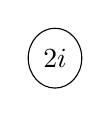
\begin{tikzpicture}\draw (0,0) ellipse (.34 and .38);\node at (0,0) {$2i$};\end{tikzpicture}}}
Par exemple, on définit le \uline{bicristal de Tate de poids \inserted{2}i}, qui est défini par le cristal de modules unité (associant à tout T sous S le Module $\underline O_T$ lui-même), et les \deleted{\unsure{appliqu}} morphismes de cristaux
\[
F=p^i\operatorname{id}_{T^i},\qquad V=p^i\operatorname{id}_{T^i}.
\]
Ainsi le bicristal de Tate de poids 2i est la puissance tensorielle i.ème du bicristal de Tate de poids 1. (NB les bicristaux de poids quelconques se multiplient tensoriellement, de \deleted{sorte} \inserted{\unsure{façon}} que les poids s'ajoutent).

1.11. Si on veut ``rendre inversible'' le bicristal de Tate $T^1$, on est obligé, qu'on le veuille ou non, de passer à une catégorie de fractions de la catégorie des cristaux de modules sur S, \inserted{[}qui entre parenthèses est une catégorie $\underline Z_p$-linéaire, (i.e. les Hom sont des $\underline Z_p$-modules ...), tout comme les catégories de p-cristaux etc qu'on en déduit\inserted{]}. Il revient donc au même de passer à une catégorie de fractions, en déclarant qu'on veut rendre notre catégorie abélienne $\underline Q$-linéaire, ou en déclarant qu'on la veut rendre $\underline Q_p$-linéaire: il faut faire le quotient par la sous-catégorie abélienne épaisse formée des objets de \deleted{p-}\unsure{torsion}, qui sont aussi des objets de p-\unsure{torsion}\inserted{\figure{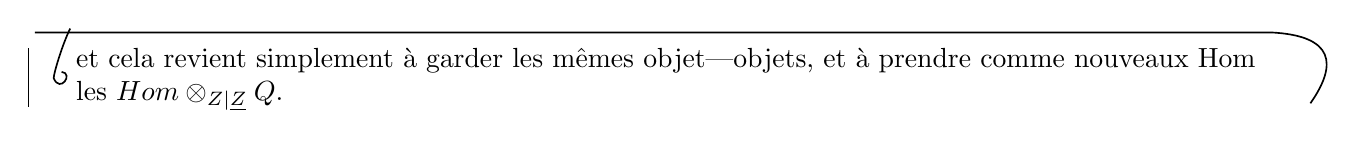
\begin{tikzpicture}
\draw[line width=.6pt] (0,0)--(15.7,0) .. controls (16.5,-.04) and (16.55,-.4) .. (16.2,-.9);
\draw[line width=.6pt] (-.08,-.2)--(-.08,-.95);
\draw[line width=.6pt] (.45,.05) .. controls (.35,-.15) and (.24,-.52) .. (.24,-.58) .. controls (.32,-.78) and (.5,-.52) .. (.34,-.5);
\node[anchor=north west,text width=15.2cm,align=left] at (.4,-.08) {et cela revient simplement à garder les mêmes \unsure{objet|objets}, et à prendre comme nouveaux Hom les $\operatorname{Hom}\otimes_{\unsure{Z|\underline Z}}Q$.};
\end{tikzpicture}}}. On trouve la catégorie des ``\uline{cristaux de modules}
\margin{8}
